\documentclass{beamer}
\usetheme{Madrid}
\usecolortheme{default}
\usepackage{graphicx}
\usepackage{amsmath}
\usepackage{hyperref}
\usepackage{tikz}

\definecolor{mycolor}{RGB}{144,180,148}
\setbeamercolor{structure}{fg=mycolor}

\title{Forces}
\subtitle{SPH-3UI Grade 11 Physics}
\date{\today}

\begin{document}

\frame{\titlepage}

% Slide 1: What is Force?
\begin{frame}
\frametitle{What is Force?}
\begin{beamercolorbox}[rounded=true, shadow=true, wd=\textwidth, sep=1em]{title}
A force is a \textbf{push} or a \textbf{pull} that can cause an object to change its motion or shape.  
\end{beamercolorbox}

\vspace{0.3cm}
In physics, force is represented by a \textbf{vector} because it has both magnitude and direction.  
For example, pushing a book sideways will have a different effect than pulling it upward.

\vspace{0.3cm}
Forces are the fundamental way that matter interacts with matter.
\end{frame}

% Slide 2: Everyday Forces Intro
\begin{frame}
\frametitle{Everyday Forces}
Example: Imagine two children playing outside with a wagon.  
One child is pulling forward on a rope tied to the front, while the other pushes from behind.

\begin{center}
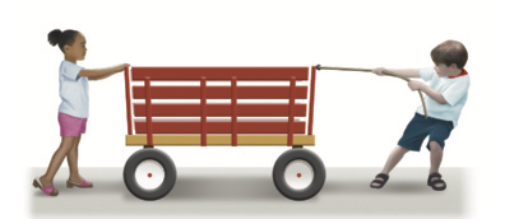
\includegraphics[width=0.8\textwidth]{wagon.png}
\end{center}

\textbf{Question:} Which forces act on the wagon? 
\end{frame}

% Slide 3: Applied Force
\begin{frame}
\frametitle{Applied Force ($\vec{F}_{app}$)}
An \textbf{applied force} results when one object is in contact with another and pushes or pulls on it.  

\begin{itemize}
\item Example: The child behind the wagon exerts an applied force forward on the wagon by pushing on the back.
\item Symbol: $\vec{F}_{app}$
\item Direction: Points away from the surface of contact.
\end{itemize}

\begin{center}
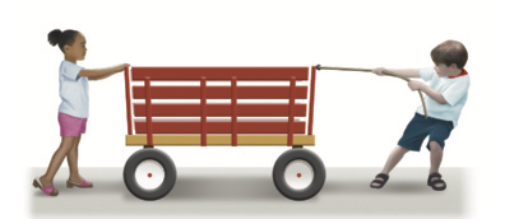
\includegraphics[width=0.5\textwidth]{wagon.png}
\end{center}
\end{frame}

% Slide 4: Tension
\begin{frame}
\frametitle{Tension ($\vec{F}_T$)}
\textbf{Tension} is a pulling force exerted on an object by a rope or string.

\begin{itemize}
\item Example: The child at the front pulls the rope, creating tension in it.
\item Symbol: $\vec{F}_T$
\item Direction: Along the rope, away from the object.
\end{itemize}

In a free-body diagram (FBD), both $\vec{F}_{app}$ and $\vec{F}_T$ start from the object and point forward.
\end{frame}

% Slide 5: Normal Force
\begin{frame}
\frametitle{Normal Force ($\vec{F}_N$)}
The \textbf{normal force} is the perpendicular contact force a surface exerts on an object.

\begin{itemize}
\item Symbol: $\vec{F}_N$
\item Always points \textbf{away from the surface.}
\item Prevents objects from falling through the surface.
\end{itemize}

\begin{center}
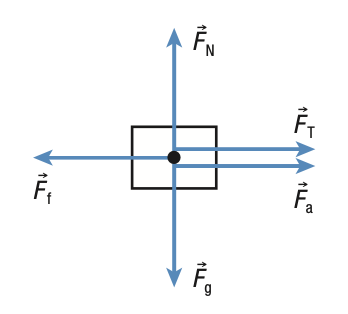
\includegraphics[width=0.45\textwidth]{FBD.png}
\end{center}
\end{frame}

% Slide 6: Friction
\begin{frame}
\frametitle{Friction ($\vec{F}_f$)}
\textbf{Friction} resists the motion or attempted motion of an object.

\begin{itemize}
\item Symbol: $\vec{F}_f$
\item Acts \textbf{parallel} to the surface.
\item Direction: Opposite to motion or attempted motion.
\item Example: If the wagon moves right, friction acts left.
\end{itemize}
\end{frame}

% Slide 7: Gravity
\begin{frame}
\frametitle{Gravitational Force ($\vec{F}_g$)}
\textbf{Gravity} (or the gravitational force) is the force of attraction between any two objects due to their mass.

\begin{itemize}
\item Symbol: $\vec{F}_g$
\item Direction: Toward the center of Earth (downward).
\item This is an \textbf{action-at-a-distance} force — it does not require contact.
\end{itemize}
\end{frame}

% Slide: How to Draw a Free-Body Diagram
\begin{frame}
\frametitle{How to Draw a Free-Body Diagram (FBD)}

A \textbf{free-body diagram (FBD)} shows an object and all the forces acting on it.  
It helps visualize how different forces interact and predict motion.

\vspace{0.4cm}

\begin{beamercolorbox}[rounded=true, shadow=true, wd=\textwidth, sep=1em]{title}
\textbf{Steps to Draw an FBD:}
\begin{enumerate}
    \item \textbf{Identify} all forces acting on the object.  
    \textit{(e.g., gravity, normal, friction, tension, applied forces)}
    \vspace{0.3cm}
    \item \textbf{Determine} the direction of each force.  
    \textit{(which way does each force act? up, down, left, right?)}
    \vspace{0.3cm}
    \item \textbf{Draw} a rectangle (the object) and arrows for each force.  
    Label each arrow with the correct symbol (e.g., $\vec{F}_g$, $\vec{F}_N$).  
    Arrows should point away from the object, and their lengths should show relative magnitudes.
\end{enumerate}
\end{beamercolorbox}

\end{frame}


% Slide 10: Net Force
\begin{frame}
\frametitle{Net Force ($\vec{F}_{net}$)}
Once all forces are identified, they combine into a single \textbf{net force}.  

\[
\vec{F}_{net} = \sum \vec{F}
\]

\begin{itemize}
\item The \textbf{net force} determines an object’s acceleration:
  \[
  \vec{F}_{net} = m\vec{a}
  \]
\item If $\vec{F}_{net} = 0$, the object stays at rest or moves at constant velocity.
\end{itemize}
\end{frame}

% --- EXAMPLE SLIDES ---

% Example 1: Book on Desk
\begin{frame}
\frametitle{Example 1: Coffee Cup at Rest on a Desk}


\vspace{0.4cm}
\textbf{Description:}  
A coffee cup rests motionless on a flat desk. \textbf{Draw the corresponding FBD.}

\vspace{0.5cm}

\begin{columns}
\column{0.48\textwidth}
\centering
\textit{System Diagram:}\\[0.2cm]
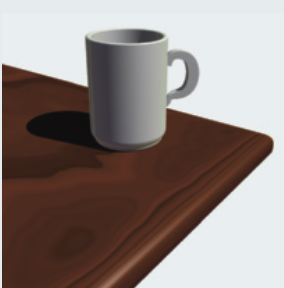
\includegraphics[width=0.95\linewidth]{cupEX1.png}


\column{0.48\textwidth}
\centering
\pause
\textit{Free-Body Diagram (FBD):}\\[0.2cm]
%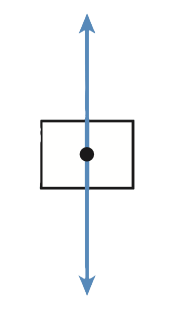
\includegraphics[width=0.55\linewidth]{ex1FBD.png}
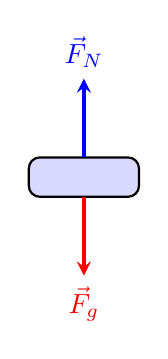
\begin{tikzpicture}[scale=1, thick, >=stealth]

% object (book)
\draw[fill=blue!15, rounded corners] (-0.7,0) rectangle (0.7,0.5);

% normal force (up)
\draw[->, blue, line width=1.2pt] (0,0.5) -- (0,1.5)
    node[above] {$\vec{F}_N$};

% gravitational force (down)
\draw[->, red, line width=1.2pt] (0,0) -- (0,-1)
    node[below] {$\vec{F}_g$};

\end{tikzpicture}

\end{columns}

\end{frame}


% Example 2: George Springer
\begin{frame}
\frametitle{Example 1: Baseball Player Sliding}


\textbf{Description:}  
George Springer has just put the Blue Jays in the lead with a home run in the 7th inning of Game 7 of the ALCS. Just as he's about to score, for the sake of grade 11 physics students, he decides to slide into home plate so they can analyze the forces acting on him. 
\vspace{0.2cm}

\begin{columns}
\column{0.48\textwidth}
\centering
\textit{System Diagram:}\\[0.2cm]
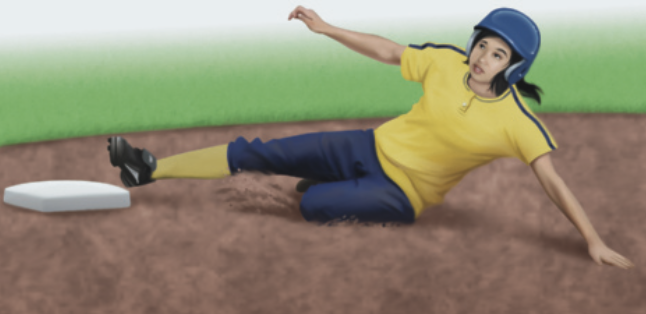
\includegraphics[width=0.95\linewidth]{ex2.png}


\column{0.48\textwidth}
\centering
\pause
\textit{Free-Body Diagram (FBD):}\\[0.2cm]
%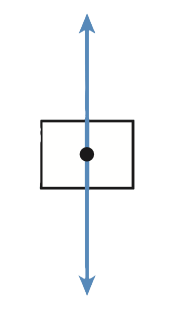
\includegraphics[width=0.55\linewidth]{ex1FBD.png}
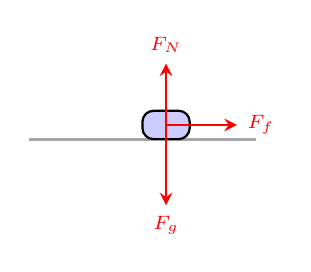
\begin{tikzpicture}[scale=1.2, thick, >=stealth]
  % draw ground
  \draw[gray!70, line width=1pt] (-1.2,0) -- (1.2,0);

  % draw box for george springer (the "system")
  \draw[fill=blue!20, rounded corners] (0,0) rectangle (0.5,0.3);

  % draw forces
  % gravity
  \draw[->, red, line width=1pt] (0.25,0.15) -- (0.25,-0.7) node[below] {\scriptsize $F_g$};
  % normal
  \draw[->, red, line width=1pt] (0.25,0.15) -- (0.25,0.8) node[above] {\scriptsize $F_N$};
  % friction (points to the right if sliding left)
  \draw[->, red, line width=1pt] (0.25,0.15) -- (1,0.15) node[right] {\scriptsize $F_f$};

\end{tikzpicture}


\end{columns}
\pause
\begin{beamercolorbox}[rounded=true, shadow=true, wd=\textwidth, sep=0.8em]{title}
\textbf{Note:} There’s no $F_\text{A}$ because he’s not continuously pushing on anything to keep moving. 

\end{beamercolorbox}

\end{frame}


% Example 3: Vector Addition of Forces
\begin{frame}
\frametitle{Example 3: Determine the Net Force}

\textbf{Description:} The floor exerts a normal force of 36 N [up] on a stationary chair. The force of gravity on the chair is 36 N [down]. Draw the FBD of the chair and use the FBD to determine the net force on the chair. 

\vspace{0.3cm}

\begin{columns}
\column{0.48\textwidth}
\centering

\begin{beamercolorbox}[rounded=true, shadow=true, wd=\textwidth, sep=0.8em]{title}
\textbf{Step 1:} Draw the FBD of the object. \\
\textbf{Step 2:} Identify which directions are positive. \\
\textbf{Step 3:} Add the forces on each axis to determine the net force. 
\end{beamercolorbox}

\vspace{0.4cm}
\column{0.48\textwidth}
\centering
\pause
\textit{Free-Body Diagram (FBD):}\\[0.2cm]
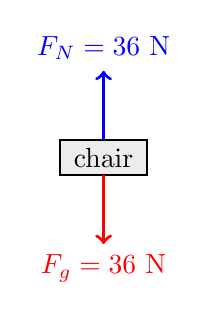
\begin{tikzpicture}[scale=1.1, thick]
  % draw the object
  \draw[fill=gray!15] (-0.5,-0.2) rectangle (0.5,0.2);
  \node at (0,0) {chair};

  % forces
  \draw[->, blue, line width=1.2pt] (0,0.2) -- (0,1) node[above] {$F_N = 36~\text{N}$};
  \draw[->, red, line width=1.2pt] (0,-0.2) -- (0,-1) node[below] {$F_g = 36~\text{N}$};
\end{tikzpicture}
\end{columns}

\pause
\centering
\[
\begin{aligned}
\vec{F}_{\text{net}} &= \vec{F}_N + \vec{F}_g \\
\vec{F}_{\text{net}} &= (+36~\text{N}) + (-36~\text{N}) \\
\vec{F}_{\text{net}} &= 0~\text{N}
\end{aligned}
\]


\end{frame}

% Slide: Practice and Reference
\begin{frame}
\frametitle{Textbook & Practice}

\begin{beamercolorbox}[rounded=true, shadow=true, wd=\textwidth, sep=0.8em]{title}
\textbf{Textbook Reference:} \\
Pg. 114–121
\end{beamercolorbox}

\vspace{0.5cm}

\begin{beamercolorbox}[rounded=true, shadow=true, wd=\textwidth, sep=0.8em]{title}
\textbf{Practice Questions:}
\begin{itemize}
    \item Pg. 120 \#1–3
    \item \textit{Forces and Free-Body Diagrams Practice} worksheet
\end{itemize}
\end{beamercolorbox}


\end{frame}





\end{document}
